
\section{River at rest with varying width and topography}

This is a test if the method is well-balanced. Furthermore, we test if the wet/dry interface has been correctly treated for steep river banks. This test is taken from the work of Goutal and Maurel~\cite{GM1997}.

The initial condition is a river at rest with water depth $12.0$. Boundary conditions are solid wall. The width and topography of the river are defined as piecewise linear interpolations of the data presented in Table~\ref{tab:width_topo}.
\begin{table}
	\centering
	\caption{River width and topography (see Goutal and Maurel~\cite{GM1997}).}
	\begin{tabular}{c|c|c}	\hline
	$x$&      topography  & width                                                       \\	\hline \hline
0 &0& 40 \\
50 &0& 40\\
100 &2.5& 30\\
150 &5& 30\\
250 &5& 30\\
300 &3& 30\\
350 &5& 25\\
400 &5& 25\\
425 &7.5& 30\\
435 &8& 35\\
450 &9& 35\\
470 &9& 40\\
475 &9& 40\\
500 &9.1& 40\\
505 &9& 45\\
530 &9& 45\\
550 &6& 50\\
565 &5.5& 45\\
575 &5.5& 40\\
600 &5& 40\\
650 &4& 30\\
700 &3& 40\\
750 &3& 40\\
800 &2.3& 5\\
820 &2& 40\\
900 &1.2& 35\\
950 &0.4& 25\\
1000 &0& 40\\
1500 &0& 40 \\ \hline
	\end{tabular}
	
	\label{tab:width_topo}
\end{table} 
The analytical solution is the river at rest, that is, $w=12.0$ and $u=v=0$.

\subsection{Results}


Current version of \anuga{} might not treat the wet/dry interface appropriately. The following three figures show the stage, $x$-momentum, and $x$-velocity respectively, after we run the simulation for some time. We should see excellent agreement between the analytical and numerical solutions if the method is well-balanced and if the wet/dry interface has been correctly treated.

\begin{figure}
\begin{center}
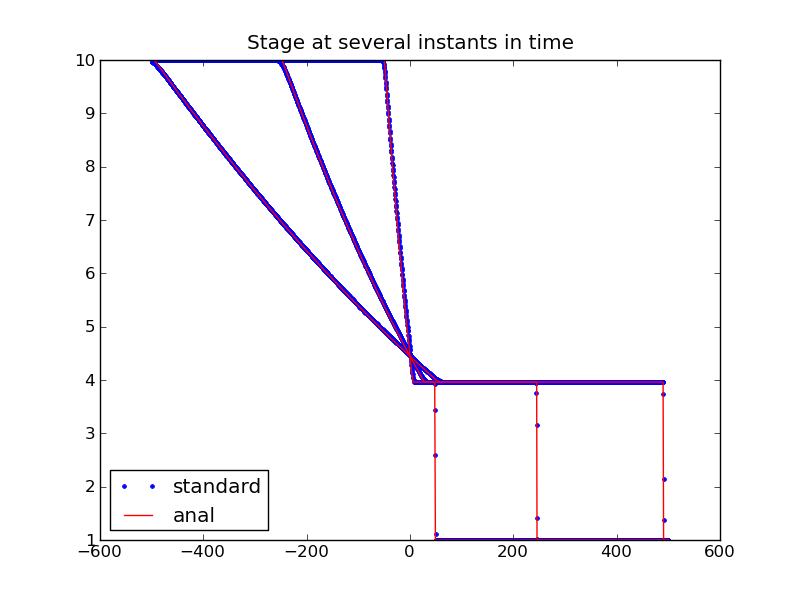
\includegraphics[width=0.9\textwidth]{stage_plot.png}
\end{center}
\caption{Stage results}
\end{figure}


\begin{figure}
\begin{center}
\includegraphics[width=0.9\textwidth]{xmom_plot.png}
\end{center}
\caption{Xmomentum results}
\end{figure}


\begin{figure}
\begin{center}
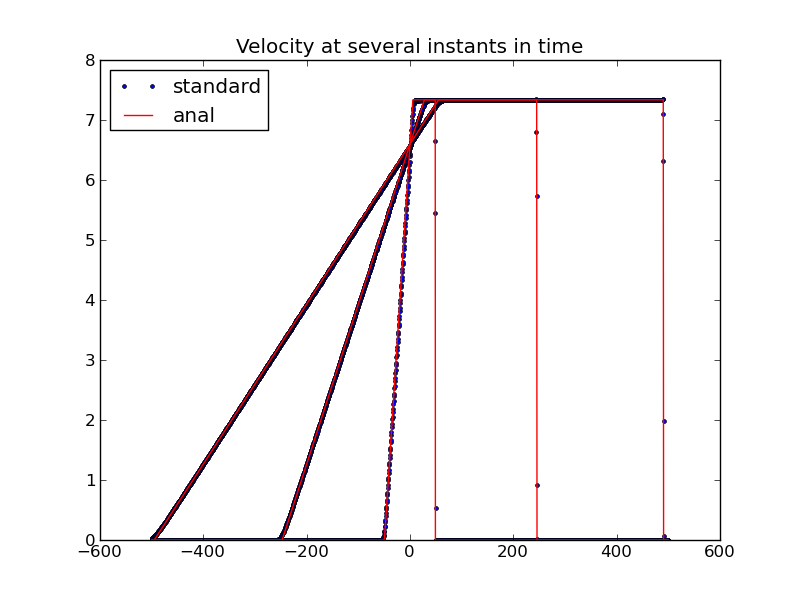
\includegraphics[width=0.9\textwidth]{xvel_plot.png}
\end{center}
\caption{Xvelocity results}
\end{figure}


\endinput
